
\chapter{Une vue générale sur le clustering hiérarchique. Ou comment introduire des \emph{a priori}. %Ou comment «~hacker~» HDBSCAN
}
\label{chap:hacker_hdbscan}

%\rouge{24 mars - 30 mars}

%Disons-le d'emblée : 
%Ce chapitre occupe une place singulière dans ce manuscrit. Il 
Ce chapitre ne présente ni nouveaux concepts théoriques fondamentaux, ni nouvelles preuves mathématiques ; il s'adresse plutôt aux ingénieurs et chercheurs curieux, désireux de décortiquer la mécanique de HDBSCAN pour l'adapter, par exemple, à des problèmes industriels spécifiques.

Comme nous l'avons vu au chapitre précédent, le succès de HDBSCAN réside dans sa capacité à extraire un clustering qui soit à la fois multi-échelle et qui gère (relativement) bien le bruit.

Nous montrons d'abord dans ce chapitre que la structure d'arbre (l'ultramétrique) est un cadre mathématique puissant qui permet d'unifier et de résoudre de manière quasi-triviale des problèmes d'optimisation (comme le $k$-Means), autrement \texttt{NP}-complets dans un cadre plus général. 
Il est possible de ``hacker'' l'étape d'extraction de HDBSCAN en substituant à sa fonction de coût statistique des \emph{a priori}. 
Nous illustrons cette démarche avec notre généralisation du Single-Linkage, {HGP-Clusterer} (HGP pour Hypergraphe-Percol'), qui sera théorisé dans la partie suivante. Nous proposons deux cas d'usage réels : la détection d'anomalies par rapport à un modèle 3D théorique (\copyright Naval Group) et la segmentation d'instance 4D sur des nuages de points LiDAR (sur le jeu de données \href{https://semantic-kitti.org/}{SemanticKITTI} \cite{SemanticKITTI}).

\Contributions{Nous adoptons une vue unificatrice du clustering hiérarchique (en intégrant le formalisme de l'analyse convexe). Nous nous appuyons ensuite sur les récents travaux de \textsc{Draganov} \etal \cite{Draganov2025} pour rappeler qu'un arbre ultramétrique simplifie drastiquement les algorithmes de clustering : le $k$-Means, \texttt{NP}-complet dans $\mathbb R^p$, y est résolu optimalement en temps de tri. 
Nous montrons comment remplacer la fonction de coût de HDBSCAN, l'excès de masse, par une fonction de coût intégrant des \emph{a priori} géométriques. Nous montrons l'efficacité de cette approche sur des nuages 3D et 4D avec notre algorithme {HGP-Clusterer} pour deux applications industrielles (détection d'anomalies sur un chantier naval et \emph{tracking} par transport optimal sur SemanticKITTI).}


\section{L'arbre comme espace de résolution : unifier le clustering}

Il existe une dichotomie historique entre les algorithmes de clustering cherchant des centroïdes (comme le $k$-Means) et les algorithmes agglomératifs (comme le Single-Linkage). Néanmoins, ces deux visions peuvent être unifiées sous le prisme de l'optimisation convexe.

\subsection{Formalisation convexe du problème de clustering}
\label{sec:convex_clustering}

Le \emph{convex clustering} \cite{hocking2011clusterpath, chi2015splitting} reformule le clustering comme un problème d'optimisation convexe global. Soit $X \in \mathbb{R}^{n \times p}$ la matrice des données observées. L'idée centrale est de relâcher la contrainte d'appartenance discrète en associant à chaque observation $x_i$ un centroïde $u_i \in \mathbb{R}^{p}$. Le clustering émerge par la coalescence de ces centroïdes en minimisant :
\[
    \min_{U \in \mathbb{R}^{n \times p}} \underbrace{\frac{1}{2} \sum_{i=1}^n \|x_i - u_i\|^2}_{\text{Fidélité (Attache aux données)}} + \gamma \underbrace{\sum_{i < j} w_{ij} \|u_i - u_j\|}_{\text{Pénalité de fusion (Régularisation)}}
    \label{eq:convex_clustering}
\]
où $\gamma \ge 0$ est un paramètre de régularisation et $w_{ij}$ des poids positifs encodant la géométrie locale. 

L'analyse de ce problème \cite{tan2015statistical} offre une perspective mécanique éclairante. En introduisant les variables duales $v_{ij}$ associées aux contraintes de différence, on obtient des conditions de capacité $\|v_{ij}\| \le \gamma w_{ij}$. Les variables $v_{ij}$ s'interprètent comme des \emph{forces de tension} s'exerçant entre les points. Deux clusters ne fusionnent ($u_i = u_j$) que lorsque l'équilibre des forces nécessite de saturer la capacité du lien $\gamma w_{ij}$. Cette structure duale révèle que le \emph{convex clustering} est en réalité une relaxation robuste du Single-Linkage\footnote{Le Single-Linkage pouvant se formuler comme un cas très particulier de ce problème \cite{tan2015statistical}.}, où la fusion ne dépend plus d'un unique point (susceptible de créer un effet de chaînage) mais d'un ensemble de tensions. 

\begin{figure}[ht]
    \centering
    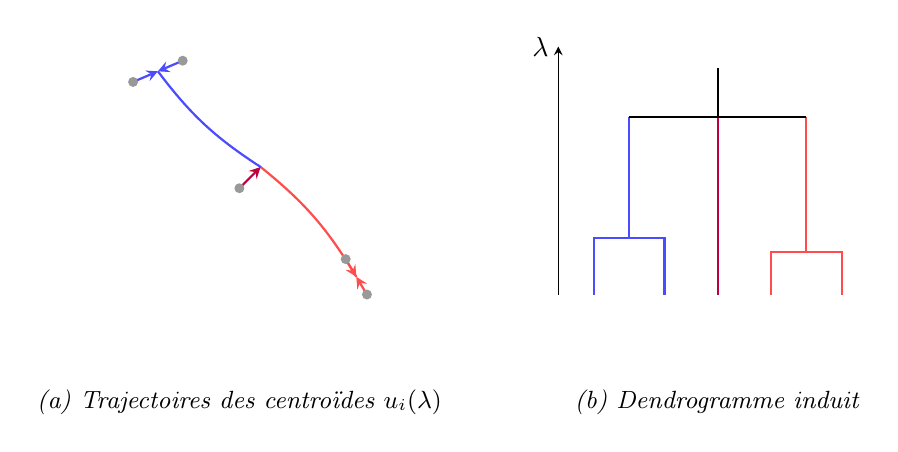
\begin{tikzpicture}[scale=0.9, >=stealth]
        % -- Panneau Gauche : Espace 2D et Trajectoires --
        \begin{scope}[local bounding box=A]
            %\draw[->, gray!40] (-0.5,0) -- (4.5,0) node[right, black] {\scriptsize Espace des features};
            %\draw[->, gray!40] (0,-0.5) -- (0,4.5);
            
            % Points de données originaux (x_i)
            \coordinate (x1) at (0.5, 3.5);
            \coordinate (x2) at (1.2, 3.8);
            \coordinate (x3) at (3.5, 1.0);
            \coordinate (x4) at (3.8, 0.5);
            \coordinate (x5) at (2.0, 2.0); % Outlier/Center

            % Points de fusion (Centroids mergés)
            \coordinate (c1) at (0.85, 3.65); % Fusion cluster haut gauche
            \coordinate (c2) at (3.65, 0.75); % Fusion cluster bas droite
            \coordinate (grand_center) at (2.3, 2.3);

            % Trajectoires (Clusterpaths)
            % Cluster 1 (Haut Gauche)
            \draw[thick, blue!70, ->] (x1) -- (c1);
            \draw[thick, blue!70, ->] (x2) -- (c1);
            \draw[thick, blue!70] (c1) to[bend right=10] (grand_center);
            
            % Cluster 2 (Bas Droite)
            \draw[thick, red!70, ->] (x3) -- (c2);
            \draw[thick, red!70, ->] (x4) -- (c2);
            \draw[thick, red!70] (c2) to[bend right=10] (grand_center);
            
            % Outlier
            \draw[thick, purple, ->] (x5) -- (grand_center);

            % Points initiaux
            \foreach \p in {x1,x2,x3,x4,x5} \fill[gray!80] (\p) circle (2pt);
            
            %\node[font=\footnotesize] at (0.2, 3.8) {$x_1$};
            %\node[font=\footnotesize] at (4.1, 0.5) {$x_4$};
            
            \node[anchor=north] at (2, -0.7) {\small \textit{(a) Trajectoires des centroïdes $u_i(\lambda)$}};
        \end{scope}

        % -- Panneau Droit : Dendrogramme --
        \begin{scope}[xshift=6.5cm, yshift=0.5cm, local bounding box=B]
            % Axe Lambda
            \draw[->] (0,0) -- (0, 3.5) node[left] {$\lambda$};
            %\node[below] at (2.25,0) {\scriptsize Indices des points};
            
            % Arbre
            % Cluster 1-2 (Bleu)
            \draw[blue!70, thick] (0.5,0) -- (0.5, 0.8) -- (1.5, 0.8) -- (1.5, 0); 
            %\node[right, font=\tiny, color=black!60] at (1.5, 0.8) {Fusion locale};
            
            % Cluster 3-4 (Rouge)
            \draw[red!70, thick] (3.0,0) -- (3.0, 0.6) -- (4.0, 0.6) -- (4.0, 0); 
            
            % Branches montantes
            \draw[blue!70, thick] (1.0, 0.8) -- (1.0, 2.5); % Branche gauche
            \draw[red!70, thick] (3.5, 0.6) -- (3.5, 2.5); % Branche droite
            \draw[purple, thick] (2.25, 0) -- (2.25, 2.8);   % Point 5 (outlier)
            
            % Fusion globale
            \draw[thick] (1.0, 2.5) -- (3.5, 2.5); % Fusion (1-2) et (3-4)
            \draw[thick] (2.25, 2.5) -- (2.25, 2.8) -- (2.25, 3.2); % Racine finale

            % Labels
            %\node[below, font=\scriptsize] at (0.5,0) {1};
            %\node[below, font=\scriptsize] at (1.5,0) {2};
            %\node[below, font=\scriptsize] at (2.25,0) {5};
            %\node[below, font=\scriptsize] at (3.0,0) {3};
            %\node[below, font=\scriptsize] at (4.0,0) {4};
            
            \node[anchor=north] at (2.25, -1.2) {\small \textit{(b) Dendrogramme induit}};
        \end{scope}
    \end{tikzpicture}
    \caption{Illustration du principe du Convex Clustering. (a) Dans l'espace des données, l'augmentation de la pénalité $\gamma$ force les centroïdes à se déplacer physiquement (\textit{shrinkage}) vers les zones de densité locale. (b) La séquence temporelle de ces coalescences permet de reconstruire l'arbre hiérarchique.}
    \label{fig:convex_clustering_viz}
\end{figure}

En faisant varier $\gamma$, la séquence temporelle de coalescence des centroïdes permet de reconstruire un arbre hiérarchique (voir l'illustration en \Fig~\ref{fig:convex_clustering_viz}).

\subsection{Quand les problèmes \texttt{NP}-complets deviennent triviaux}

Si la recherche de centroïdes optimaux (comme dans le $k$-Means ou le $k$-Median) est connue pour être un problème NP-complet dans l'espace euclidien $\mathbb R^p$ pour $k \ge 2$, la situation change radicalement dès lors que la métrique est une ultramétrique, c'est-à-dire que l'on dispose d'une structure d'arbre.

En théorie des graphes, de nombreux algorithmes \texttt{NP}-complets sur des graphes généraux deviennent de complexité quasi-linéaire lorsque le graphe est un arbre. Il en va de même pour le clustering, comme l'ont montré \textsc{Draganov} \etal dans leur récent papier \cite{Draganov2025}.

\begin{Resultat}{Résolution optimale du $k$-Means sur les hiérarchies ultramétriques \cite{Draganov2025}}{draganov_kMeans}
Pour n'importe quelle hiérarchie, les objectifs de clustering recourant aux centres (tels que le $k$-Means, $k$-Median, ou $k$-Centre) peuvent être résolus \emph{de manière optimale}. Mieux encore, l'ensemble complet des solutions optimales pour tout $k \in \IntervalleEntiers{1 ; n}$ peut être trouvé en un temps équivalent à celui d'un tri, soit $\mathcal{O}(n \log n)$. %Enfin, les solutions de ces clusterings optimaux forment elles-mêmes une hiérarchie.
\end{Resultat}

Ce résultat est une excellente nouvelle : une fois que nous disposons d'un bon arbre hiérarchique, il n'y a plus à s'en remettre à une heuristique : la hiérarchie elle-même devient un espace dans lequel chercher \emph{très rapidement} la solution qui nous intéresse (qu'il s'agisse d'un $k$-Means optimal ou de toute autre exploration guidée selon le problème).


\section{«~Hacker~» HDBSCAN : l'exploration de l'arbre hiérarchique}

Revenons à HDBSCAN. Pour extraire un clustering ``à plat'' depuis la hiérarchie, l'algorithme calcule l'excès de masse (\Def[def:excess_mass]) de chaque nœud, puis propage cette valeur de bas en haut.


\begin{figure}[!ht]
    \centering
    \begin{tikzpicture}[
        >=stealth,
        treenode/.style={
            rectangle split,
            rectangle split parts=2,
            draw=blue!60!cyan,
            line width=1.2pt,
            rounded corners=4pt,
            rectangle split part fill={blue!60!cyan, white},
            text width=2.6cm,
            align=center,
            font=\sffamily,
            inner sep=1.2ex
        }
    ]

    % Nœud Parent
    \node[treenode] (parent) at (0, 0) {
        \textcolor{white}{\textbf{Père}}
        \nodepart{two}
        loss(Père)
    };

    % Nœuds Enfants
    \node[treenode] (child1) at (-4.8, -3) {
        \textcolor{white}{\textbf{Fils 1}}
        \nodepart{two}
        loss(Fils 1)
    };

    \node[treenode] (child2) at (-1.6, -3) {
        \textcolor{white}{\textbf{Fils 2}}
        \nodepart{two}
        loss(Fils 2)
    };

    \node[treenode] (child3) at (1.6, -3) {
        \textcolor{white}{\textbf{Fils 3}}
        \nodepart{two}
        loss(Fils 3)
    };

    % Points de suspension
    \node[font=\Huge, text=blue!60!cyan] (dots) at (4.5, -3) {\dots};

    % Flèches
    \draw[->, blue!60!cyan, line width=1.2pt] (parent.195) to[out=195, in=90] (child1.north);
    \draw[->, blue!60!cyan, line width=1.2pt] (parent.250) to[out=250, in=90] (child2.north);
    \draw[->, blue!60!cyan, line width=1.2pt] (parent.290) to[out=290, in=90] (child3.north);
    \draw[->, blue!60!cyan, line width=1.2pt] (parent.345) to[out=345, in=90] (dots.north);

    % Accolade
    \draw[decorate, decoration={brace, amplitude=10pt, mirror}, blue!60!cyan, line width=1.2pt]
        ([xshift=-0.2cm, yshift=-0.3cm]child1.south west) -- 
        ([xshift=0.4cm, yshift=-0.3cm]child1.south -| dots.east)
        coordinate[midway, below=12pt] (brace_center);

    % Texte Comparaison
    \node[anchor=north, font=\sffamily, align=center] (comp) at ([yshift=-0.2cm]brace_center) {
        \textbf{Comparaison~:} loss(Père) \emph{vs.} loss(\{Fils $i$\}$_i$)
    };
    
    % Flèche pointant vers le texte
    \draw[->, blue!60!cyan, line width=1.2pt] (brace_center) -- (comp.north);

    \end{tikzpicture}
    \caption{Le mécanisme de sélection d'un cluster. L'architecture de HDBSCAN compare la perte (\emph{loss}) d'un nœud parent à la somme de celles de ses enfants. En jouant sur la fonction de coût, l'on peut introduire des \emph{a priori}.}
    \label{fig:hack_hdbscan_loss}
\end{figure}



La décision prise au niveau du nœud parent $C_{\mathrm{Père}}$ s'écrit de manière générique :
\[
    \text{Si } \mathrm{loss}(C_{\mathrm{Père}}) < \sum_{i} \mathrm{loss}(C_{\mathrm{Fils}, i}) \implies \text{Conserver le nœud parent, sinon continuer d'explorer.}
\]

Dans le cas de l'excès de masse de HDBSCAN, il suffit de poser $ \mathrm{loss}(C) = - \tilde E(C)$.
L'excès de masse est un critère purement statistique, aveugle à la géométrie. Si nous substituons cette fonction de coût par une évaluation personnalisée au problème rencontré (l'alignement d'une structure, le volume maximal attendu d'un objet, ou la conformité à un modèle 3D), l'algorithme se transforme en un extracteur guidé géométriquement. 

Nous illustrons cette approche sur deux applications pratiques, en utilisant {HGP-Clusterer} (notre généralisation du Single-Linkage aux interactions d'ordre supérieur, qui sera définie formellement dans la partie suivante, voir \Def[def:hgp_clusterer]) pour générer l'arbre hiérarchique de base.


\section{Application I : Détection d'anomalies 3D guidée par un modèle théorique (\copyright Naval Group)}

La première application concerne un problème de structuration de données industrielles : le nettoyage d'un nuage de points LiDAR dans un chantier naval (travail réalisé sur une partie du projet Inria Startup Studio de Marie \textsc{Aspro}, en collaboration avec elle).

\subsection{Le problème}
Nous disposons en entrée :
\begin{enumerate}
    \item D'un modèle 3D théorique du chantier naval (les boîtes englobantes des infrastructures attendues).
    \item D'un nuage de points 3D brut, fortement bruité, acquis par un capteur LiDAR (la réalité du chantier).
\end{enumerate}
L'objectif est d'isoler les objets physiques présents dans le nuage mais absents du modèle théorique (ex. : des casques, des tuteurs, des câbles ou des outils). 

%L'approche non-supervisée classique (basée sur l'excès de masse) est ici inopérante. Les anomalies (comme un casque posé sur le pont du navire) sont physiquement en contact avec la structure principale. La densité locale y est forte, et le critère statistique fusionnera systématiquement l'anomalie avec le navire.

\subsection{L'exploration guidée}
Nous construisons la hiérarchie du nuage LiDAR avec {HGP-Clusterer}. Lors de la navigation dans l'arbre, notre fonction de coût n'évalue plus la densité, mais utilise le modèle 3D théorique comme \emph{a priori}.

Pour un nœud donné de l'arbre, la fonction calcule sa ``{pureté}'' géométrique (par exemple à l'aide de l'index de \textsc{Gini} \cite{IndexGini}) : on vérifie la proportion de ses points qui tombent à l'intérieur ou à l'extérieur des limites du modèle théorique.
\begin{itemize}
    \item Si un nœud parent est hybride (il contient à la fois des points de la structure valide du navire et une anomalie qui y est accollée), la fonction de coût force la scission de l'arbre pour isoler la composante étrangère.
    \item Dès qu'une branche atteint un seuil adéquat de pureté (la grande majorité de ses points sont situés ou bien hors du modèle théorique, ou bien peuvent être rattachés au modèle), l'algorithme valide le cluster (en tant qu'anomalie ou en tant qu'objet conforme au modèle 3D).
\end{itemize}

\subsection{Le post-traitement}
Les occultations inhérentes aux acquisitions LiDAR ont la fâcheuse tendance à fragmenter un objet réel (un câble caché par un poteau par exemple) en plusieurs sous-clusters. 
Nous ne cherchons pas à forcer une partition parfaite absolue au moment de l'exploration de l'arbre. À la place, un post-traitement très simple est appliqué : nous calculons les boîtes englobantes des anomalies extraites, et en parcourant leur matrice d'adjacence on fusionne les fragments d'un même objet. Les points de bruits résiduels piégés dans ces boîtes sont ensuite absorbés.

\begin{figure}[!ht]
    \centering
    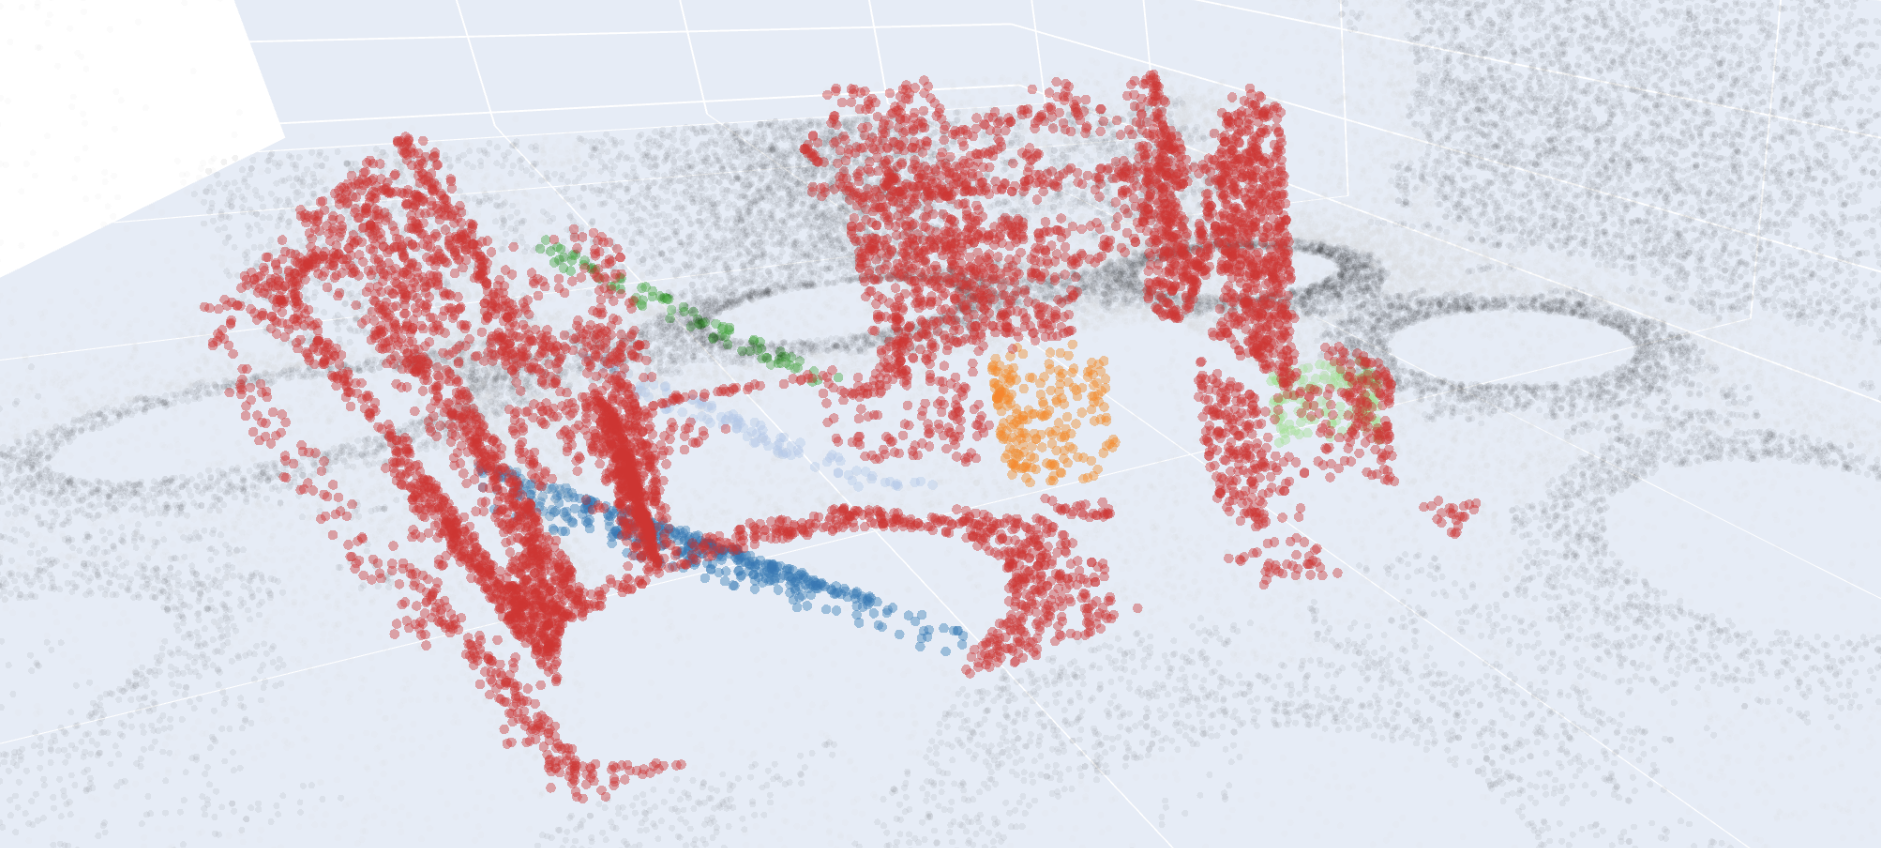
\includegraphics[width=0.9\textwidth]{../img/ResultatMarieBenchmark.png}
    \caption{Détection d'anomalies sur un \emph{benchmark} synthétique (\copyright Naval Group) de 2\,000\,000 de points. L'injection du modèle 3D théorique (bien identifié en \textcolor{red}{rouge}) comme \emph{a priori} géométrique dans la fonction de coût lors de l'exploration de la hiérarchie produite par HGP-Clusterer permet d'isoler parfaitement les objets étrangers (trois tuteurs, deux cubes ; chacun avec sa couleur). Le « hors-champ » apparaît en gris.}
    \label{fig:shipyard_anomaly}
\end{figure}

Cette approche montre que l'injection d'une supervision géométrique faible (la simple indication spatiale du modèle 3D théorique) directement dans la fonction de coût de l'arbre hiérarchique offre une solution robuste, interprétable, et qui s'affranchit totalement des coûteuses méthodes d'apprentissage profond (\emph{training-free}).

\paragraph{\emph{Nota bene} :} Le test montré en \Fig~\ref{fig:shipyard_anomaly} est un ``petit'' nuage \emph{synthétique} de 2\,000\,000 de points. Pour des raisons de confidentialité, nous ne pouvons pas montrer les résultats sur des données réelles (avec des nuages de l'ordre de 10\,000\,000 de points), situations autrement plus difficiles, mais où notre algorithme s'en tire bien mieux que toutes les autres méthodes essayées par Marie \textsc{Aspro} ainsi que la même \emph{baseline} où HDBSCAN est substitué à notre HGP-Clusterer.


\section{Application II : {Segmentation d'instance 4D} sur SemanticKITTI}

La seconde application s'attaque à la segmentation d'instance (ou segmentation panoptique) « 4D » (c'est-à-dire avec suivi des objets d'intérêt, des \emph{instances}, au cours du temps), évaluée sur le jeu de données \href{https://semantic-kitti.org/}{SemanticKITTI} \cite{SemanticKITTI}. L'objectif est de détecter (segmenter) spatialement et suivre temporellement des objets dynamiques (véhicules, piétons, \emph{etc}.).

Nous reprenons ici les idées récentes de la littérature scientifique qui montrent qu'il est possible d'obtenir l'« état-de-l'art » une fois la sémantique du nuage connue, et sans apprentissage additionnel. Comme le soulignent \textsc{Sautier} \etal \cite{Sautier2025}, une approche de clustering pur permet d'obtenir une très bonne segmentation d'instance sur chaque trame (\emph{frame} en anglais). 

De plus, pour le suivi au cours du temps (\emph{tracking} en anglais), \textsc{Oh} \etal \cite{Oh2025} ont montré plus récemment encore qu'une association géométrique globale est extrêmement efficace.

\subsection{La méthode}
%Nous allons faire mieux grâce à HGP-Clusterer ! 
Notre processus de \emph{streaming} se divise en deux étapes (voir un exemple en \Fig~\ref{fig:SemanticKITTI_frame60_HGP} et le résultat sur les 200 premières trames la séquence 08 de SemanticKITTI en \Fig~\ref{fig:comparaison_SemanticKITTI}) :
\begin{enumerate}
    \item \textbf{Segmentation spatiale 3D.} Pour chaque trame et pour chaque classe d'intérêt, nous générons une hiérarchie avec HGP-Clusterer. Lors de l'exploration de cette hiérarchie, notre fonction de coût est guidée par la sémantique (\emph{a priori} sur les dimensions attendues selon la classe de l'objet). Si, par exemple, un nœud décrit un amas de la taille de deux véhicules fusionnés par la densité, le volume physique aberrant force l'algorithme à scinder le nœud.
    Cette première passe, assez proche dans l'idée du travail de \textsc{Sautier} \etal \cite{Sautier2025}, fournit non pas un clustering du nuage de points mais une forêt hiérarchique, un ensemble d'arbres hiérarchiques dont la racine représente le cluster qu'aurait choisi l'algorithme sur une unique trame. Cette forêt est ensuite passée au \emph{tracker}. 
    \item \textbf{Suivi temporel (\emph{tracking} 4D).} Le suivi d'une trame à l'autre est assuré par l'utilisation du transport optimal \cite{Peyre2019}. L'état cinématique des objets (centroïdes et dimensions) est lissé au cours du temps par un filtre de \textsc{Kalman} \cite{FiltreKalman}. Pour associer les prédictions de la trame $t-1$ aux détections géométriques de la trame $t$, nous calculons un plan de transport optimal entre les pistes de la trame $t-1$ extrapolées au temps $t$ et le nuage correspondant au temps $t$. Nous reprenons alors l'exploration de la forêt obtenue à l'étape précédente pour obtenir un appariement optimal entre les pistes extrapolées et les clusters potentiels au temps $t$. Tout arbre n'ayant aucun de ses nœuds associé à une piste déjà confirmée crée une nouvelle piste potentielle. Le problème de transport optimal est déséquilibré \cite{Chizat2018UOT} (\emph{unbalanced} ; d'une trame à l'autre, une instance n'a pas forcément le même nombre de points) et régularisé par l'entropie, convexifiant ainsi le problème et permettant le recours à des algorithmes hautement parallélisables de type Sinkhorn \cite{Cuturi2013Sinkhorn}.
\end{enumerate}

\begin{figure}[!h]
    \centering
    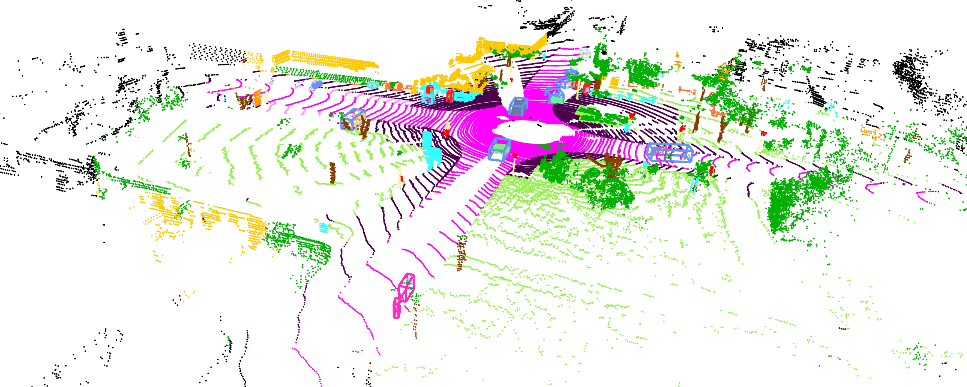
\includegraphics[width=0.8\textwidth]{Manuscrit these Louis Hauseux/img/SemanticKITTI_frame60_HGP.png}
    \caption{Résultat de notre méthode sur la trame 60, séquence 08, de SemanticKITTI. Chaque piste est repérée par sa boîte englobante (une couleur par classe d'objets). Noter les deux cyclistes (boîtes roses) en bas, bien séparés quoique proches (et ce grâce au suivi par transport optimal, quand le clustering avec \emph{a priori} géométriques les avait fusionnés).\label{fig:SemanticKITTI_frame60_HGP}}
\end{figure}


\begin{figure}[!htbp]
    \centering
    % Première sous-image
    \begin{subfigure}[b]{0.45\textwidth}
        \centering
        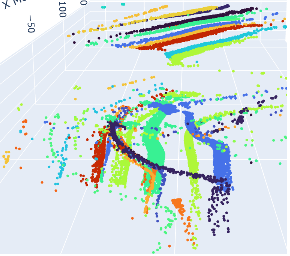
\includegraphics[height=140px]{Manuscrit these Louis Hauseux/img/SemanticKITTI_200frames_GT.png}
        \caption{Vérité terrain}
        \label{fig:ground_truth}
    \end{subfigure}
    \hfill % Ajoute un espace entre les deux images
    % Deuxième sous-image
    \begin{subfigure}[b]{0.45\textwidth}
        \centering
        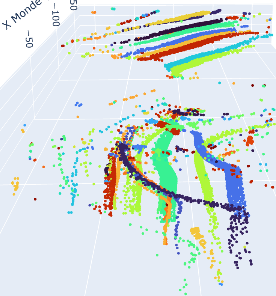
\includegraphics[height=140px]{Manuscrit these Louis Hauseux/img/SemanticKITTI_200frames_HGP.png}
        \caption{Notre méthode}
        \label{fig:SemanticKITTI_200frames}
    \end{subfigure}
    
    \caption{Segmentation panoptique 4D sur les 200 premières trames de la séquence 08 de SemanticKITTI. Les instances spatiales sont projetées en 2D (\emph{Bird-Eye-View}), le temps $t$ est repéré sur le troisième axe. Chaque piste suivie reçoit une couleur et produit donc comme une traînée avec le temps. À gauche, la vérité terrain. À droite, le résultat de notre méthode (clustering hiérarchique guidé par la géométrie + transport optimal déséquilibré régularisé par l'entropie).}
    \label{fig:comparaison_SemanticKITTI}
\end{figure}

Les résultats (\Fig~\ref{fig:comparaison_SemanticKITTI}) montrent que les pistes principales sont bien détectées et suivies au cours du temps. L'algorithme présente encore quelques faiblesses pour un transfert vers l'industrie : la gestion du bruit, des petites pistes lointaines, et des occlusions, rendant certaines pistes ``clignotantes'' notamment. Le temps de réponse est aussi un problème : de l'ordre de la seconde pour l'instant lorsqu'une version industrielle impose de pouvoir traiter plusieurs trames à la seconde (dix trames par seconde avec les capteurs qui ont servi à l'établissement de SemanticKITTI) .



\Synthese{Ce chapitre illustre la puissance et la flexibilité du clustering hiérarchique. L'arbre ultramétrique %n'est pas seulement le résultat d'un algorithme agglomératif ; c'
est un espace dans lequel des problèmes $\NP$-complets complexes peuvent être résolus très rapidement de manière optimale (comme le $k$-Means \cite{Draganov2025}). 

%En comprenant que la sélection des clusters dans un arbre, telle qu'implémentée dans HDBSCAN, peut être décorrélée du seul critère statistique d'excès de masse, 
Lors de l'exploration de l'arbre hiérarchique, nous avons montré qu'il est possible d'injecter des \emph{a priori} géométriques (le modèle 3D théorique, les dimensions physiques). Les résultats obtenus avec notre algorithme {HGP-Clusterer} sur la détection d'anomalies LiDAR et la segmentation panoptique 4D valident cette approche pragmatique et \emph{training-free}.

Cependant, la robustesse de ces applications s'appuie fondamentalement sur la qualité de l'arbre généré. Or, comme souligné précédemment, le {Robust Single-Linkage} (moteur de HDBSCAN) ne reflète pas la topologie des densités $K$-NN lorsque $K \ge 2$. Il est donc impératif de pallier ces faiblesses. C'est l'objet de la partie suivante, où l'on y définit notre méthode HGP-Clusterer.
%dans la partie suivante, de définir formellement le cadre théorique de notre {HGP-Clusterer}.
}